% !TeX document-id = {1220ecc9-4e94-4765-8bf8-191a286a997a}
\documentclass[
	ngerman,
	parskip=half,
	headsepline,
	fontsize=12pt,
	DIV=13,
	listof=leveldown,
	]{scrreprt}

\KOMAoptions{DIV=last}

\usepackage[utf8]{inputenc}
\usepackage[T1]{fontenc}

\usepackage{titling}

% Basic Look & Feel
\usepackage{babel}
\usepackage{lmodern}
\usepackage{microtype}
\usepackage{graphicx}
\usepackage{xspace}
\usepackage[xindy, nonumberlist, nogroupskip]{glossaries}
\usepackage{csquotes}
\usepackage{enumitem}
\usepackage{float}
\usepackage{gensymb, siunitx}
\sisetup{per-mode=symbol, binary-units=true}

% References
\usepackage[hyphens]{url}
\usepackage[hidelinks,linktoc=all]{hyperref}
\usepackage{cleveref}
\usepackage[backend=biber, style=trad-plain]{biblatex}
\addbibresource{bibliography.bib} 

% Tables
\usepackage{array}
\usepackage{booktabs}
\usepackage{multirow}

% Enable shell-escape
% !TeX TXS-program:compile = txs:///pdflatex/[--shell-escape]

%--------------------------------------------------------------------------------
%\lohead[]{}
%\rohead[]{\leftmark}
%\cohead[]{}

%
%captionsetup{format=plain,indention=2em}

%\makeglossaries
%\setacronymstyle{long-short}
%\loadglsentries{}

% Titel
\author{Jakob Birkenfeld, Josef Herbert, Sergej Zuyev}
\title{Datenbank ACM - Inhalt, Datenbankaufbau und Recherche}
\subject{Kommunikation in wissenschaftlicher und beruflicher Arbeit WS2017}
\titlehead{
\includegraphics[width=\linewidth]{Logo_THM}}
\date{\today}

\graphicspath{{img/}}



%--------------------------------------------------------------------------------

\makeindex
\makeglossaries

\begin{document}
	\begin{titlepage}
		\maketitle
	\end{titlepage}
	
	\begin{abstract}
		In diesem Dokument wird die wissenschaftliche Datenbank \textbf{ACM} beschrieben und nach dem Datenbankfahrplan der UB Chemnitz \cite{resource:dbf} bewertet.
		
		In this document the scientific database \textbf{ACM} is described and evaluated according to \cite{resource:dbf}.
	\end{abstract}

	\clearpage
	
	\pagenumbering{Roman}
		\tableofcontents
		\listoffigures	
	\pagenumbering{arabic}
	
	\clearpage
	
	\chapter{Einführung}	
	Literaturdatenbanken ermöglichen die Recherche von Informationen im \textit{Deep Web} und somit den umfassenden Überblick über Publikationen einer Institution. Standardsuchmaschinen, wie z.B. \textit{Google}, erreichen diese Informationen oftmals nicht. Daher ist eine Nutzung von Literaturdatenbanken sehr sinnvoll. Die Digitalisierung hat dabei die früher üblichen Zettelkästen abgelöst und vereinfacht die Literaturrecherche enorm. Umfangreiche Suchfunktionen, teilweise sogar mit Volltextsuche, stehen dabei dem Benutzer zur Verfügung. Die in einer solchen Fachdatenbank erhaltenen Medientypen sind nicht auf Bücher beschränkt, sondern beinhalten oftmals auch Zeitschriften und multimediale Elemente. \cite{resource:wld}
	\ \\
	\ \\
	Die ACM (\textit{Association for Computing Machinery}) gilt mit ihrer Gründung im Jahr 1947 als erste wissenschaftliche Gesellschaft für Informatik \cite{resource:wacm}. Sie regt zum Dialog unter Forschern, Lehrenden und Fachleuten an \cite{resource:aacm}. Das geschieht durch:
\begin{itemize}
\item jährlich mehrere Fachkonferenzen.
\item \textit{sog. Special Interest Groups}, kurz \textit{SIG}. Diese Gruppen sind thematisch gegliedert und besitzen jeweils ein eigenes Leitungsgremium. Dadurch ist eine Spezialisierung der Mitglieder auf bestimmte Fachgebiete möglich.
\item regelmäßige Veröffentlichungen. Dazu zählen Magazine, Journals und Transactions.
\item eine digitale Bibliothek (\textit{Digital Libary}). Diese stellt Publikationen bis zum Gründungsjahr der ACM entgeltlich online zur Verfügung. Sie gilt als weltweit größte Sammlung ihrer Art.
\end{itemize}
Dieser Bericht erläutert und diskutiert die Möglichkeiten, die sich durch Nutzung der wissenschaftlichen Datenbank der ACM (\textit{Digital Libary}) eröffnen.
\ \\
\begin{figure}[ht]
\begin{minipage}[b]{0.55\linewidth}
\centering

\includegraphics[width=\textwidth]{img/acmLogo.PNG}
\caption{Das Logo der ACM.}
\end{minipage}
\end{figure}
% Bildquelle: \url{http://www.acm.org/images/top-menu/acm_logo_tablet.svg}

	\chapter{Methoden}
	Um einen möglichst umfassenden Überblick über die Datenbank der ACM zu erhalten, wird der Datenbankfahrplan der UB Chemnitz \cite{resource:dbf} verwendet. Dieser vereinfacht die Untersuchung der Möglichkeiten einer bibliographischen Datenbank anhand gezielter Fragestellungen.
\ \\	
\ \\
	Außerdem wird eine selbstständig und eine unselbstständig erschienene wissenschaftliche Publikation in der Datenbank recherchiert und untersucht. Der Schwerpunkt liegt dabei auf dem grundsätzlichen Aufbau und Inhalt der Datensätze.
	
	
	\chapter{Ergebnisse}
	In diesem Kapitel soll anhand dem vorher erwähnten Datenbankfahrplan der UB Chemnitz \cite{resource:dbf} die \textsl{ACM Digital Library} analysiert und beschrieben werden.
		\ \\
		\ \\
		Zunächst zum Inhalt: Es handelt sich um eine Datenbank mit Volltextsuche, die es dem Benutzer ermöglicht, in verzeichneten Werken nach Schlagwörtern und Wortfolgen sowie Kombinationen zu suchen. Die angebotenen Medientypen sind vielfältig: Neben Büchern, Zeitschriften, Magazinen, Protokollen und Kongressberichten finden sich auch Videoaufzeichnungen von Fachkonferenzen.
		\ \\
		Eine eigene Abteilung bildet die \textsl{Computing Literature}, die sich ausschließlich mit Büchern und Berichten der Informatik befasst.
		\ \\
		\ \\
		In der Datenbank kann über die einfache und die erweiterte Maske gesucht werden:
		\begin{itemize}
		\item Die einfache Suche ist direkt von der Startseite der \textsl{ACM Digital Library} zugänglich. Sie besteht nur aus einer Textbox, die einfache Stichwortsuchen etc. entgegennimmt.
		\item In der erweiterten Suche können bestimmte Felder für die Suche spezifiziert werden. Zur Auswahl stehen hier verschiedene Felder wie Autor, Titel, Erscheinungsjahr, Volltext und andere Kriterien. Es könne beliebig viele Kriterien zur Verfeinerung der Suche kombiniert werden. Die Suche ist grafisch aufbereitet; so müssen die Suchkriterien nicht per Hand in einem bestimmten Syntax eingegeben werden. Dadurch können vom Benutzer auch boolsche Suchoperatoren wie UND, ODER sowie NICHT noch einfacher nachvollziehbar angewandt werden. Für fortgeschrittene Benutzer ist aber selbstverständlich auch direkte Suche mittels \textit{query syntax} möglich. In diesem Format lässt sich eine Suche leichter extern speichern, ohne ein Bildschirmfoto zu erstellen und dieses dann nachzubauen.
		\end{itemize}
		\ \\
		Eine erfolgte Suche kann nachträglich nach Relevanz, Publikationsdatum, Anzahl der Zitationen oder Downloads sortiert werden. Ebenso kann auch weiter nach Personen (Autor, Editor, Reviewer...), Publikationen, oder auch nach Konferenzen (bei Protokollen und Berichten) gefiltert werden. Diese Funktionalität befindet sich in der rechten Seitenleiste. Sehr interessant ist auch der dort gezeigte Graph: So lässt sich ablesen, in welchem Jahr es wie viele Publikationen gegeben hat, die den Suchkriterien entsprechen. Gerade weil die \textit{ACM} als erste wissenschaftliche Gesellschaft für Informatik gilt, lassen sich durch diese Funktion auch historische Betrachtungen anstellen.
		\ \\
		\ \\
		Die Suchergebnisse können weiter exportiert werden nach \textit{bibtex}, \textit{endnote}, \textit{acmref} oder \textit{csv}. Ebenso ist die Einbindung von Citavi möglich. Somit ist eine einfache Referenzierung und Zitierung im eigenen Literaturverwaltungsprogramm möglich.
		\ \\
		\ \\
		Über eine Anmeldefunktion ist es ebenso möglich, seine Suchanfragen zu speichern und zu verwalten, um später erneut darauf zurückgreifen zu können.	
\\\
\\\
Als Beispiel hier noch die erweiterte Suche einer unselbstständigen Quelle. Zu finden ist der Artikel ,,Analyzing and predicting the impact of CAD algorithm noise on FPGA speed performance and power". Nun ist dem Sucher allerdings der genaue Titel nicht mehr bekannt und sucht in der allgemeinen Suche. Hier werden dann allerdings 4,268 Suchergebnisse zurückgegeben. Das gesuchte Werk befindet sich hier etwa auf der fünften Ergebnisseite. 
\begin{figure}[ht]
\centering
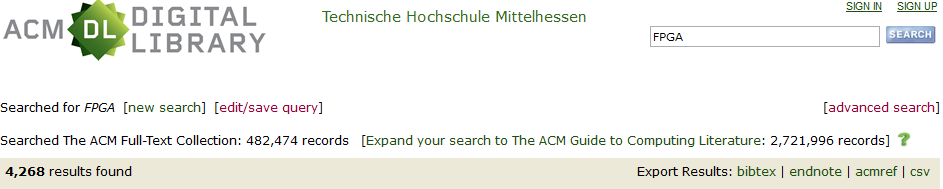
\includegraphics[width=\textwidth]{img/Suche_FPGA.PNG}
\caption{einfache Suche nach ,,FPGA''}
\end{figure}
Im folgenden soll anhand der erweiterten Suche das Suchergebnis präzisiert werden. Zunächst wird für Titel das Schlagwort ,,FPGA'' eingegeben und als Autor soll unter anderem ,,Shum'' gelistet sein.
Die Suche wurde hier Einschließlich aber nicht ausschließlich gewählt (matches any) alternativ wäre die ausschließliche Suche (matches all) möglich, sowie die ausschließende suche (matches none) möglich.
Sofern der Autor bekannt ist, reduziert sich das Suchergebnis somit auf nur nun mehr 2 Suchergebnisse.
\begin{figure}[ht]
\centering
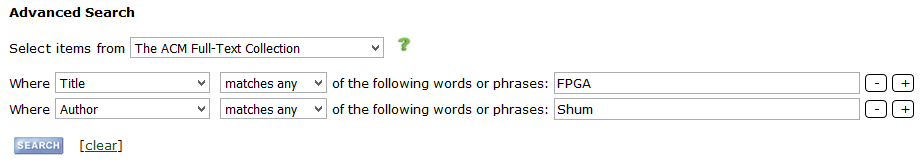
\includegraphics[width=\textwidth]{img/Suche_FPGA-Shum.PNG}
\caption{erweiterte Suche}
\end{figure}
So kann man die Suche auf einfache Art stark eingrenzen, sofern Bibliografische Eigenschaften wie Autor, Erscheinungsdatum etc bekannt sind.
\newpage
Als Beispiel für eine selbstständig erschienene Quelle wird ein aktuelles Buch herangeführt: \textit{Shared-Memory Parallelism Can Be Simple, Fast and Scalable}, erschienen im Jahr 2017. Der Aufbau dieses Datensatzes unterscheidet sich eigentlich nur in der Schnellübersicht von dem einer unselbständig erschienenen Quelle.
\ \\
\begin{figure}[ht]
\centering
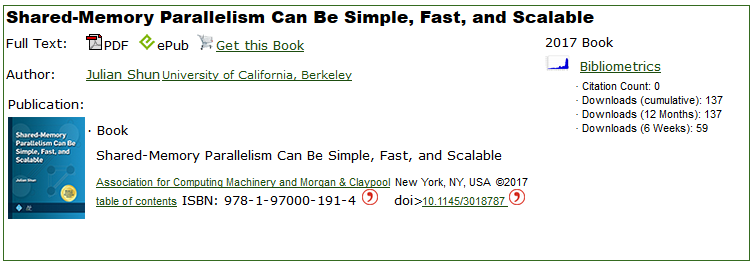
\includegraphics[width=\textwidth]{img/seq.PNG}
\caption{Schnellübersicht des Buches \textit{Shared-Memory Parallelism Can Be Simple, Fast and Scalable}}
\end{figure}
\ \\
So findet sich dort die Formulierung \textit{Publication} statt \textit{Published in}. Der Medientyp an der linken Seite ist auch entsprechend angepasst: \textit{Book} statt \textit{Article}. Außerdem finden sich keine Seitenangaben, die den zugehörigen Bereich auf einen Teil des Werkes beschränken.
	\chapter{Diskussion}	
	
	Die \textsl{ACM Digital Library} erlaubt es, komfortabel Inhalte aus dem Themengebiet der Informationstechnologie zu suchen. Die Volltextsuche ermöglicht dem Nutzer, nicht nur über Metadaten sondern auch über Stichwörter in den Inhalten relevante Werke zu finden; erweiterte Suchfunktionen stellen auch fortgeschrittene Benutzer zufrieden. Weitere Funktionen wie die Filterung der Suchergebnisse nach zahlreichen Kriterien und umfangreiche Exportmöglichkeiten sind ebenfalls positive Eigenschaften der Datenbank. 
	
	Ein geringfügiges Defizit ist allerdings die konservative Oberfläche, welche einem neuen Benutzer Schwierigkeiten bereiten könnte. Außerdem gehört es zum guten Ton, dem Benutzer eine Hilfsfunktionalität anzubieten, welche im Webportal nicht aufzufinden war. Möglicherweise wurde darauf verzichtet, da die erwartete Zielgruppe ohnehin IT-affin ist.
	Eine mobile Anwendung für gängige Smartphones wird angeboten und intensiv auf Webpräsenz beworben. Diese Anwendung bietet in der getesteten freien Version eine rudimentäre Suchfunktion und hat auf den ersten Blick nur einen geringen Mehrwert gegenüber der Webpräsenz. Vorstellbar wäre ein Szenario, bei welchem die Recherche am klassischen Arbeitsplatz stattfindet, und mit der mobilen Anwendung die gefundenen und über das Benutzerkopnto synchronisierten Inhalte während einer Reise gelesen werden können.
	
	Vor einer Recherche ist zu beachten, dass die \textbf{ACM}-Datenbank ausschließlich auf Inhalte verweist, die von \textbf{ACM} veröffentlicht wurden und  eine Verbindung zu Informationstechnologien aufweisen. Für den Beginn der allgemeinen oder domänenübergreifenden Recherchen ist die \textsl{ACM Digital Library} zu speziell, sodass allgemeine Datenbanken vorzuziehen sind.
	
	\chapter{Eigenständigkeitserklärung}
	
	Wir versichern hiermit ehrenwörtlich, dass ich die vorliegende Arbeit selbstständig und ohne Benutzung anderer als der angegebenen Hilfsmittel angefertigt habe. Alle Stellen, die wörtlich oder sinngemäß aus veröffentlichten oder unveröffentlichten Quellen entnommen worden sind, sind als solche kenntlich gemacht. Diese Arbeit lag in gleicher oder ähnlicher Form noch keiner anderen Prüfungsbehörde vor und wurde bisher noch nicht veröffentlicht.
	
	Friedberg, den \today
	
	
	\rule[-0.2cm]{5cm}{0.5pt}
	
	\textsc{\theauthor} 

	
	
	
	\printbibliography
\end{document}
